\documentclass[hidelinks,a4paper]{article}
\usepackage[margin=2cm]{geometry}
\usepackage{natbib}
\usepackage{latexsym}
\usepackage{url}
\usepackage{hyperref}
\hypersetup{
    colorlinks = true,
    citecolor = blue
}
\usepackage{epsfig}
\usepackage{graphicx}
\usepackage{amssymb}
\usepackage{amsmath}
\usepackage{hyperref}
\usepackage{amsthm}
\usepackage{amstext}
\usepackage{lineno}
\usepackage[english]{babel}
\usepackage{multicol}
\usepackage{ragged2e}

\DeclareMathOperator*\mslim{ms-lim}
\usepackage[printwatermark]{xwatermark}
\usepackage{xcolor}
\newwatermark[allpages,color=lightgray!50, angle=45,scale=3,xpos=0,ypos=0]{DRAFT}
% Add and remove packages as necessary for your manuscript.
\linespread{1.66} % NEED to UNCOMMENT
% All text should be double-spaced
% with occasional exceptions for tables. 
\raggedright
\setlength{\parindent}{0.5in}

\setcounter{secnumdepth}{0}
\pagestyle{empty}

\renewcommand{\section}[1]{%
\bigskip
\begin{center}
\begin{Large}
\normalfont\scshape #1
\medskip
\end{Large}
\end{center}}

\renewcommand{\subsection}[1]{%
\bigskip
\begin{center}
\begin{large}
\normalfont\itshape #1
\end{large}
\end{center}}

\renewcommand{\subsubsection}[1]{%
\vspace{2ex}
\noindent
\textit{#1.}---}

\renewcommand{\tableofcontents}{}
    
\bibpunct{(}{)}{;}{a}{}{,}  % this is a citation format command for natbib

\begin{document}
\begin{flushright}
Version dated: \today
\end{flushright}
\bigskip
\noindent RH: PHYLOGENETIC MULTIPLE IMPUTATION
\bigskip
\medskip
\begin{center}
% Insert your title:
\noindent{\Large \bf IMPUTING CONTINUOUS DATA USING PHYLOGENETIC INFORMATION}
\bigskip
\linebreak
\noindent {\normalsize \sc Patrik Drhlik\textsuperscript{1,2} and Simon P. Blomberg\textsuperscript{1}}\\ % need to fix accent on Drhlik
\noindent {\small
\textit{\textsuperscript{1}School of Biological Sciences, University of Queensland, St. Lucia, Queensland, 4072, Australia.}\\ E-mail: s.blomberg1@uq.edu.au}
\end{center}
\medskip
\begin{center}
\noindent{\small
\textit{\textsuperscript{2}Faculty of Mechatronics, Informatics and Interdisciplinary Studies, Technical University of Liberec, 461 17 Liberec, Czech Republic.}\\E-mail: patrik.drhlik@tul.cz}
\end{center}

\medskip
%\vspace{1in}

%\linenumbers
\justify
\subsubsection{Abstract}
Biological databases are often sparse which makes their analyses more difficult. One of the most plausible solutions of dealing with sparse databases is using multiple imputation (MI). MI has already been implemented and is usually a part of most standard statistical softwares. These methods do not use the potential of phylogenies though and do not preserve phylogenetic signal in traits. In this paper, we present new MI methods that preserve phylogenetic signal after the imputation process. These methods were developed in R and based on methods used in R mice package. These methods have been previously suggested as a possible way of improving MI but have not been implemented yet.
\\
\noindent (Keywords: Multiple imputation, mice, missing data, phylogenetic signals, phylogenetic imputation, R statistical software)\\
\newpage
\begin{multicols}{2}

\section{Possible titles}
IMPUTING CONTINUOUS DATA USING PHYLOGENETIC INFORMATION

IMPUTING CONTINUOUS DATA INCORPORATING PHYLOGENETIC INFORMATION

IMPUTING CONTINUOUS DATA INCORPORATING PHYLOGENIES

PHYLOGENETIC IMPUTATION IN R

\section{Notes on observations}
phnorm - lambda\\
tree size x trait size - more or less the same\\
tree size x tree shape - it seems that pure birth trees give the best results, one sided trees are the worst\\
tree size x lambda transform - the bigger the lambda before imp, the bigger after, seems to be working slightly better for larger trees\\
tree size x miss data mech - slightly better when mcar\\
tree size x miss data level - it works better when the tree is larger and has more missing data (higher the level, more missing data there is)\\

trait size x tree size - more or less the same\\
trait size x tree shape - pure birth the best\\
trait size x lambda transorm - decreasing trend while more traits\\
trait size x miss data mech - not enough measures in mcar\\
trait size x miss data level - better when more missing data, gets worse with more traits\\

tree shape - all variable share the same trend: pure birth best, balanced worse, one sided worst\\

\newpage

\section{Introduction}
Biological and ecological databases contain vast amounts of data. Unfortunately, these databases are very sparse for various reasons. Even the largest plant trait database has a really sparse data matrix \cite{kattge2011try}. All of this makes analyses more difficult. There are several methods that can handle the missing data problem. They span from the easiest like casewise deletion \cite{allison2001missing} to complex procedures like multiple imputation \cite{allison2001missing,miRubin}. Methods like a multivariate imputation by chained equations (MICE) have been already successfully implemented \cite{Buuren2011} and are part of a standard software nowadays. None of these methods incorporates the use of phylogenetic information to preserve the phylogenetic signal \cite{blomberg2003testing}. It has been suggested \cite{swenson2014phylogenetic,Garland2000} but not yet implemented. In this paper, we present an extension to R mice package \cite{Buuren2011} that provides a multiple imputation method where imputed data do not lose the phylogenetic information.

\subsection{Why is missing data a problem?}
Everybody who is interested in missing data knows this quote from R.A. Fisher -- ``The best solution to handle missing data is to have none.''. This solution would be a nice way to handle the problem but it is almost impossible to be achieved in real world problems. Any kind of a survey is very likely to have missing data because of the human nature -- either we don't want to respond to some questions or we simply forget that there is a second page.

Several problems arise when a data set has missing data. If we use a simple approach where we delete all observations that contain missing data (casewise deletion or complete case analysis), we abandon a lot of data. Imagine a data set that has a hundred observations of ten traits. Thirty of these observations only lack one of the traits and you would have to exclude whole observations because of that even though the other nine traits were fully observed. That leads to a bias in the analysis and decreases a statistical power of the model.

\subsection{Missing data assumptions}
There are several missing data assumptions \cite{allison2001missing,Donders06} that need to be taken in account before handling the data. For a well explaining graphical example about the differences between these mechanisms, see \cite{Nakagawa2008}. The strongest assumption is that the data are \emph{missing completely at random} (MCAR). That means that the missingness is not related neither to dependent nor independent variables. If we can assume that this mechanism is present then even a casewise deletion method can produce unbiased estimates.

A weaker but still strong assumption is \emph{missing at random} (MAR). This mechanism says that the missingness of the data may depend on the input variable. In other words, there might be a threshold above which the probability of missing data is very high. That might for example be the case when people do not fill in the amount of money they make in a survey. They might not want to share that information if they make too much.

The weakest assumption is \emph{missing not at random} (MNAR). This mechanism assumes that the missing data in a response variable depends on the response variable itself. Which means that it is something that is not observed. This assumption is said to be \emph{non-ignorable} as opposed to MCAR and MAR which are \emph{ignorable} \cite{allison2001missing}. When the mechanism is identified as MNAR, the analysis is usually very difficult and often requires a unique approach \cite{Buuren2011}.

\subsection{Missing data approaches}
We are going to describe a few methods (but not all) that are used in the missing data problems.

The easiest way to handle missing data is a method called casewise deletion (sometimes also complete case analysis or listwise deletion) \cite{allison2001missing,Donders06}. You need to delete all observations with missing data and then start your analysis. When it comes to a standard software, this is often a default option how to handle missing data. As mentioned before, this method would not produce biased estimates under the MCAR assumption. That is usually not the case and you should therefore consider different methods.

There is a whole group of method that we call \emph{imputations}. Those are either single or multiple. When using a single imputation method, we impute values to fill the gaps in data sets. After this process, the data set looks like it never had missing values in the first place. We do not try to guess the actual missing values, just to replace them to make the analysis possible. We can either replace them by \emph{constant values} (imputing a mean value), \emph{random values} (randomly choosing one value from observed values) or we can \emph{nonrandomly derive} them (conditional mean imputation, regression imputation). All of these methods are discussed in \cite{Donders06}.

Multiple imputation (MI) is the most sophisticated and praised method for handling missing data \cite{allison2001missing,Schafer1997}. Single imputation creates one imputed data set whereas MI creates more (usually 3--10, \cite{Donders06}). We then do our statistical analysis on each of the newly created imputed data sets and combine all the results together. The combining process is called \emph{pooling} \cite{Buuren2011}. This produces statistically powerful and unbiased results, although some more work needs to be done when the missingness is under the MNAR assumption \cite{Buuren2011}. Imputations may sometimes create implausible values (e.g. negative body mass) but can be easily handled by a method suggested by \cite{Hussain2010}.

\subsection{Advantages of MI}
\begin{itemize}
	\item{generality}
	\item{ease of implementation}
	\item{incorporation of imputation error}
\end{itemize}

\subsection{Previous MI implementations}
R already has several several MI packages that can be used to deal with missing data. \emph{mice} \cite{Buuren2011} and \emph{Amelia} \cite{ameliaR} packages are simple to use than \emph{mi} package \cite{miR}. \emph{mi} on the other hand has more thorough MI diagnostics. The main reason we chose to extend \emph{mice} was that it is very easily extensible. It already has a lot of MI methods that a user can use and to add a new one is as easy as creating a function and naming \texttt{mice.impute.***}, where \texttt{***} stands for the new method name.

\subsection{Problem}
The problem of existing \emph{mice} methods is that all of them treat data as independent. That means that we do not take in account possible similarities among individual observations in the imputation process. Because of that, traits tend to lose their phylogenetic signal \cite{blomberg2003testing} which makes the imputation less accurate. Therefore we implemented and present new MI methods which preserve phylogenetic signal that extend the already mentioned R \emph{mice} package.

\section{Methods}
Our methods are based on the idea of incorporating phylogenetic variance--covariance matrices that can be obtained from phylogenetic trees. There are several possible ways to implement these methods as suggested by \cite{swenson2014phylogenetic} and the one we have chosen is to make use of a \emph{generalized linear model} \cite{Garland2000}. A different solution would be to implement it using \emph{phylogenetic eigenvectors} but it has been suggested that \emph{generalized linear models} perform better in the imputation \cite{rohlf2001comparative,freckleton2002phylogenetic}. We have created a new R package called \emph{phylomice} that contains our phylogenetic imputation methods and we propose that it should serve as a base package for other phylogenetic imputation methods to come in the future.

\subsection{phnorm}
The method called \emph{phnorm} stands for \emph{phylogenetic norm}. It is based on the \emph{mice.impute.norm} (\emph{norm}) function from the \emph{mice} package which imputes data using \emph{Bayesian linear regression analysis}. \cite{Buuren2011} notes that using \emph{norm} for all columns is similar to the \emph{NORM} method by \cite{Schafer1997}.

The regression problem can be written as

\begin{equation}
Y = \beta X + \epsilon,
\end{equation}

as noted by \cite{martins1997phylogenies}.

\emph{norm} method uses a simple linear model to draw $\beta$ parameter estimates that can be described as

\begin{equation}
\hat{\beta} = (X^T X)^{-1} X^T y,
\end{equation}

whereas \emph{phnorm} uses a generalized linear model to do that

\begin{equation}
\hat{\beta} = (X^T \Sigma^{-1} X)^{-1} X^T \Sigma^{-1} y,
\end{equation}

where $\Sigma$ is the phylogenetic variance--covariance matrix. Imputed values are estimated as

\begin{equation}
\hat{Y} = \hat{\beta} X + \epsilon,
\end{equation}

where the error term has a following distribution

\begin{equation}
\epsilon \sim N(\mu, \sigma^2 c_h).
\end{equation}

As \cite{Garland2000} describes in the appendix B, if $c_{ih}$ denotes a shared branch length between species $i$ and $h$ then $\Sigma_{ih}$ is a vector of values $c_{ih}$ for all species $i$ other than $h$. $c_{hh}$ stands for the total branch length of species $h$. Following equations then describe the mean of the error distribution and a part of a variance $c_h$

\begin{equation}
\mu = \Sigma^{'}_{ih} \Sigma^{-1} (X - \bar{x}),
\end{equation}

\begin{equation}
c_h = c_{hh} - \Sigma^{'}_{ih} \Sigma^{-1} \Sigma_{ih}.
\end{equation}

\subsection{phpp}
This method is based on a phylogenetic permutation model described by \cite{lapointe2001generalized}. The model creates a transition probabilities matrix from the phylogenetic tree and imputes already existing values based on other species relation.

\subsection{Simulation}
We simulated our proposed methods by setting different combinations of parameters. Specifically, we observed how the methods behave when we change a \emph{tree size} (which equals the number of species), \emph{trait size}, \emph{tree shape}, \emph{$\lambda$ transformation} parameter and a \emph{missing data mechanism} with a certain \emph{amount of missing data}. We tested our \emph{phnorm} and \emph{phpp} methods along with the \emph{norm} method from the \emph{mice} package for comparison.

The simulations were done for each combination of our input variables (described in table \ref{table:inputVariables}) and consisted of the following steps:

\begin{enumerate}
	\item{Set simulation parameters}
	\item{Generate tree}
	\item{Generate data}
	\item{Analyse data}
	\item{Generate missing values}
	\item{Impute missing values}
	\item{Analyse data after imputation}
\end{enumerate}

\end{multicols}
\begin{table}
	\centering
	\begin{tabular}{ | l | c | c | c | c | c |}
		\hline
		Variable name & 1st val & 2nd val & 3rd val & 4th val & 5th val \\
		\hline
		Tree size & 32 & 64 & 128 & 256 & 512 \\
		Trait size & 2 & 5 & 10 & 15 & - \\
		Tree shape & balanced & left & pure birth & - & - \\
		$\lambda$ transform & 0 & 0.5 & 0.8 & 1 & - \\
		Missing data mechanism & MAR & MCAR & - & - & - \\
		Missing data level & 1 & 2 & 3 & - & - \\
		Methods & norm & phnorm & phpp & - & - \\
		\hline
	\end{tabular}
	\footnotesize
	\caption{List of simulation parameters and their values. We tested every combination of parameters in this table.}
	\label{table:inputVariables}
\end{table}

\begin{multicols}{2}
First thing after setting the parameters was to generate a tree. Trees were specified by a number of tips and a shape. Examples of simulated tree shapes are shown in figure \ref{fig:treeShapes}. Balanced and left trees were generated using the \emph{ape} package \cite{paradis2004ape}, while the pure-birth trees were generated with the \emph{phytools} package \cite{revell2012phytools}.

In the second step, we generated our data. Data dimensions were defined by the \emph{tree and trait} size. To ensure that the data contains any phylogenetic signal, we modified the tree we generated in the first step using the specified $\lambda$ parameter. With this new tree, we created each trait under the Brownian motion \cite{revell2012phytools}.

We analysed our data and saved the following information for each trait: mean, median, mode, standard deviation, $\lambda$ value and $K$ value. The next step was to create some gaps in the data. We decided to only test missing data in one of the traits. We have simulated two missing data mechanism - MCAR and MAR, both of them in three levels. Levels of MCAR were simply corresponding to the percentage of missing data, where level 1 was 10\%, level 2 was 50\% and level 3 was 80\%. These values were randomly sampled which means that there is no relationship with other traits. Missing data in the MAR mechanism were related to the values of the first trait with a probability $e^{-k |x_1|}$, where $x_1$ was a value of the first trait and $k$ the parameter governing the strength of the relationship between the two traits. $k$ was set to 0.3, 0.8 and 1.3 for levels 1, 2 and 3, respectively.

We proceeded to the imputation after that. We created 5 imputed data sets in each simulation and we set the \texttt{maxit} parameter of the \emph{mice} function to 100. We also specified the currently simulated method and filled the \texttt{psi} parameter for \emph{phnorm} and \emph{phpp} and also the \texttt{psiinv} parameter for \emph{phnorm}. \texttt{psi} is the variance--covariance matrix obtained from the phylogenetic tree in \emph{phnorm} and a matrix with cophenetic distances (\cite{sneath1973numerical}) in \emph{phpp}. \texttt{psiinv} is just an inverse of \texttt{psi} needed only for the \emph{phnorm} method. It needs to be calculated and passed to \texttt{mice} before, because it can be computationally expensive and it would have been calculated several times if we inversed \texttt{psi} inside \texttt{phnorm}.

Last step after the imputations finished was to analyse the data again and record the same parameters as we did before we made gaps in the data.

\end{multicols}

\begin{figure}
	\centering
	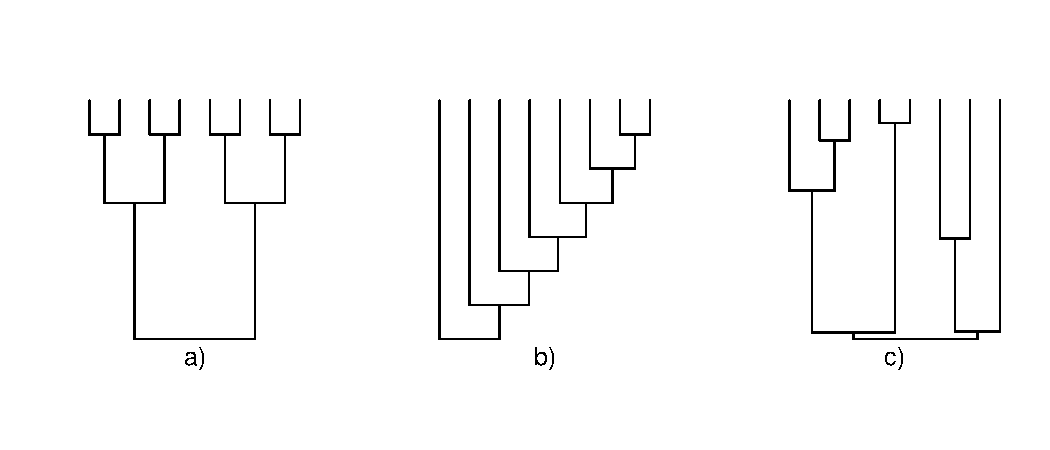
\includegraphics{graphics/trees.pdf}
	\caption{Tree shapes used in simulations -- a) balanced tree, b) one sided tree (left), c) pure-birth tree.}
	\label{fig:treeShapes}
\end{figure}

\begin{multicols}{2}

Output variables
time
imputation time
\emph{following were measured before and after imputation}
column mean
column mode
column median
column sd
$\lambda$ value
$K$ value

\subsection{Note on performance}

\subsection{Other methods extension proposal}

\section{Results}

\section{Discussion}

\section{Funding}
This research was supported by the University of Queensland, Australian Research Council grant, Erasmus Mundus NESSIE program and Student Grant Competition of Technical University of Liberec.

\section{Acknowledgments}
Thanks to S Rathnayake and ???? for insightful comments on previous drafts of this manuscript.

\renewcommand{\refname}{
\bigskip
\begin{center}
\begin{Large}
\normalfont\scshape References
\medskip
\end{Large}
\end{center}
}

\bibliographystyle{mee}
\bibliography{library}

\end{multicols}

\appendix
\renewcommand{\theequation}{A1.\arabic{equation}}
\setcounter{equation}{0}
\section{Appendix 1}

\end{document}
